\documentclass[11pt,a4paper]{article}
\usepackage[T1]{fontenc}
\usepackage[margin=23mm]{geometry}
\usepackage{amsmath,amssymb,bm,graphicx,booktabs,longtable,placeins}
\usepackage[colorlinks=true,linkcolor=blue!45!black]{hyperref}
\graphicspath{{../figures/}}
\setlength{\parindent}{0pt}\setlength{\parskip}{4pt}\setlength{\emergencystretch}{2em}
\newcommand{\PredictionTable}{\begin{longtable}{llrrrrr}\toprule Set & Model & d & q & Joint & Points & Coverage\\\midrule
1 & RBF & 3.752 & 2.197 & 3.074 & 1034 & 89.4\%\\
1 & Spline & 1.434 & 1.466 & 1.450 & 1034 & 89.4\%\\
1 & LUT & 2.302 & 0.884 & 1.744 & 1034 & 89.4\%\\
1 & kA & 5.108 & 3.845 & 4.521 & 1034 & 89.4\%\\
1 & kB & 5.154 & 3.762 & 4.512 & 1034 & 89.4\%\\
1 & kC & 5.030 & 3.737 & 4.431 & 1034 & 89.4\%\\
1 & kD & 5.226 & 3.770 & 4.556 & 1034 & 89.4\%\\
1 & kE & 5.025 & 3.731 & 4.426 & 1034 & 89.4\%\\
1 & kF & 4.629 & 4.510 & 4.570 & 1034 & 89.4\%\\
1 & kG & 5.189 & 3.838 & 4.564 & 1034 & 89.4\%\\
2 & RBF & 3.999 & 2.119 & 3.200 & 1551 & 89.4\%\\
2 & Spline & 1.661 & 1.434 & 1.552 & 1551 & 89.4\%\\
2 & LUT & 2.406 & 0.926 & 1.823 & 1551 & 89.4\%\\
2 & kA & 6.469 & 4.871 & 5.726 & 1551 & 89.4\%\\
2 & kB & 7.958 & 4.192 & 6.360 & 1551 & 89.4\%\\
2 & kC & 7.926 & 4.190 & 6.339 & 1551 & 89.4\%\\
2 & kD & 6.145 & 4.266 & 5.290 & 1551 & 89.4\%\\
2 & kE & 5.761 & 4.619 & 5.221 & 1551 & 89.4\%\\
2 & kF & 5.289 & 4.840 & 5.070 & 1551 & 89.4\%\\
2 & kG & 4.617 & 4.543 & 4.580 & 1551 & 89.4\%\\
3 & RBF & 2.191 & 1.438 & 1.853 & 1654 & 90.9\%\\
3 & Spline & 1.214 & 1.206 & 1.210 & 1654 & 90.9\%\\
3 & LUT & 1.829 & 0.834 & 1.421 & 1654 & 90.9\%\\
3 & kA & 5.705 & 6.499 & 6.115 & 1654 & 90.9\%\\
3 & kB & 5.667 & 6.640 & 6.173 & 1654 & 90.9\%\\
3 & kC & 5.687 & 6.498 & 6.106 & 1654 & 90.9\%\\
3 & kD & 6.230 & 6.319 & 6.275 & 1654 & 90.9\%\\
3 & kE & 6.561 & 6.242 & 6.403 & 1654 & 90.9\%\\
3 & kF & 5.411 & 5.987 & 5.706 & 1654 & 90.9\%\\
3 & kG & 5.914 & 6.383 & 6.153 & 1654 & 90.9\%\\
4 & RBF & 0.381 & 1.214 & 0.900 & 44 & 31.0\%\\
4 & Spline & 0.943 & 1.336 & 1.156 & 44 & 31.0\%\\
4 & LUT & 0.640 & 2.938 & 2.126 & 44 & 31.0\%\\
\bottomrule\end{longtable}}
\newcommand{\CostTable}{\begin{longtable}{llrrrr}\toprule Set & Model & Terms & Coefficients & KiB & PC median in $\mu$s\\\midrule
1 & RBF & 128 & 264 & 5.16 & 26.2\\
1 & Spline & 486 & 972 & 7.98 & 103.7\\
1 & LUT & 137781 & 275562 & 2154.38 & 242.7\\
1 & kA & 6561 & 13122 & 103.89 & 103.5\\
1 & kB & 6561 & 13122 & 103.89 & 102.6\\
1 & kC & 6561 & 13122 & 103.89 & 102.1\\
1 & kD & 6561 & 13122 & 103.90 & 198.7\\
1 & kE & 6561 & 13122 & 103.91 & 193.1\\
1 & kF & 6561 & 13122 & 103.90 & 186.2\\
1 & kG & 6561 & 13122 & 103.92 & 173.8\\
2 & RBF & 128 & 264 & 5.16 & 27.1\\
2 & Spline & 486 & 972 & 7.98 & 136.8\\
2 & LUT & 137781 & 275562 & 2154.38 & 423.9\\
2 & kA & 6561 & 13122 & 103.89 & 171.2\\
2 & kB & 6561 & 13122 & 103.89 & 90.4\\
2 & kC & 6561 & 13122 & 103.89 & 88.8\\
2 & kD & 6561 & 13122 & 103.90 & 94.2\\
2 & kE & 6561 & 13122 & 103.91 & 94.7\\
2 & kF & 6561 & 13122 & 103.90 & 90.8\\
2 & kG & 6561 & 13122 & 103.92 & 171.1\\
3 & RBF & 128 & 264 & 5.16 & 13.8\\
3 & Spline & 245 & 490 & 4.17 & 69.2\\
3 & LUT & 98415 & 196830 & 1539.23 & 212.6\\
3 & kA & 6561 & 13122 & 103.89 & 90.1\\
3 & kB & 6561 & 13122 & 103.89 & 89.4\\
3 & kC & 6561 & 13122 & 103.89 & 89.9\\
3 & kD & 6561 & 13122 & 103.90 & 89.8\\
3 & kE & 6561 & 13122 & 103.91 & 90.5\\
3 & kF & 6561 & 13122 & 103.90 & 89.0\\
3 & kG & 6561 & 13122 & 103.92 & 90.0\\
4 & RBF & 128 & 264 & 5.16 & 14.1\\
4 & Spline & 245 & 490 & 4.17 & 68.1\\
4 & LUT & 137781 & 275562 & 2154.38 & 214.3\\
\bottomrule\end{longtable}}
\newcommand{\DerivativeTable}{\begin{longtable}{llrrrrrr}\toprule Set & Model & $L_{dd}$ & $L_{dq}$ & $L_{de}$ & $L_{qd}$ & $L_{qq}$ & $L_{qe}$\\\midrule
1 & RBF & 0.042 & 0.018 & 0.738 & 0.019 & 0.015 & 0.344\\
1 & Spline & 0.038 & 0.016 & 0.661 & 0.017 & 0.017 & 0.333\\
1 & LUT & 0.049 & 0.020 & 0.562 & 0.022 & 0.018 & 0.328\\
1 & kA & 0.270 & 0.195 & 3.694 & 0.186 & 0.162 & 2.508\\
1 & kF & 0.225 & 0.199 & 3.241 & 0.199 & 0.183 & 2.894\\
2 & RBF & 0.046 & 0.015 & 0.708 & 0.016 & 0.014 & 0.389\\
2 & Spline & 0.043 & 0.017 & 0.683 & 0.017 & 0.017 & 0.318\\
2 & LUT & 0.050 & 0.021 & 0.584 & 0.022 & 0.017 & 0.303\\
2 & kA & 0.236 & 0.201 & 3.265 & 0.179 & 0.163 & 2.505\\
2 & kF & 0.196 & 0.194 & 2.839 & 0.178 & 0.172 & 2.610\\
3 & RBF & 0.032 & 0.010 & 0.459 & 0.012 & 0.015 & 0.217\\
3 & Spline & 0.032 & 0.012 & 0.333 & 0.013 & 0.018 & 0.184\\
3 & LUT & 0.047 & 0.023 & 0.348 & 0.021 & 0.019 & 0.196\\
3 & kA & 0.321 & 0.286 & 4.545 & 0.286 & 0.351 & 4.218\\
3 & kF & 0.276 & 0.265 & 3.934 & 0.279 & 0.304 & 4.124\\
\bottomrule\end{longtable}}
\newcommand{\DifferenceTable}{\begin{tabular}{lrrrr}\toprule Set & RBF & Spline & kA & kF\\\midrule
1 & 2.674 & 1.819 & 4.216 & 4.359\\
2 & 2.989 & 1.952 & 5.707 & 5.122\\
3 & 1.912 & 1.668 & 6.217 & 5.870\\
\bottomrule\end{tabular}}
\newcommand{\ReconstructionTable}{\begin{tabular}{lrrrrr}\toprule Set & RBF & Spline & LUT & kA & kF\\\midrule
1 & 2.724 & 1.513 & 0.527 & 4.321 & 4.007\\
2 & 2.738 & 1.540 & 0.601 & 4.247 & 3.806\\
3 & 1.693 & 1.006 & 0.458 & 4.033 & 3.828\\
\bottomrule\end{tabular}}
\newcommand{\ResultSummary}{On the matched excitation tests, joint RMSE for Sets 1/2/3 is 3.074/3.200/1.853 mVs for RBF; 1.450/1.552/1.210 mVs for Spline; 1.744/1.823/1.421 mVs for LUT. The spline has the smallest joint flux error among these three full-input candidates in all three current datasets; the Gaussian model has the shortest supplied MATLAB evaluation time. The spline payload is 7.98/7.98/4.17 KiB, compared with 2154.38/2154.38/1539.23 KiB for the full LUT. This is an accuracy/storage/runtime tradeoff, not an established application pass criterion. The processed artifact has a different ranking and only 44 supported test points out of 142; it cannot establish physical or temperature generalization. Upper-boundary groups have zero accepted predictions because extrapolation is disabled, rather than an extrapolation accuracy result.}

\title{\Large Coefficient-Based Stator Flux Maps\\Gaussian RBFs, Cubic Tensor Splines and Lookup Tables\\with Physical-Coordinate Derivatives}
\author{Flux Map Research Study}\date{24 October 2026}
\begin{document}\maketitle
\begin{abstract}
Compact coefficient representations of two stator flux linkages are identified while retaining three active inputs. Shared Gaussian radial basis functions and cubic tensor-product B-splines are compared with a full three-current lookup table and seven existing excitation-coordinate reductions. Three acquisition datasets use separate fitting, validation and whole-excitation-group test partitions. Model sizes are selected without test data. Measured-reference flux errors, differences from lookup tables, derivative diagnostics, storage and PC evaluation cost are distinguished. A processed two-temperature-band artifact is a secondary implementation exercise with unverified acquisition provenance. The study identifies candidates for target-hardware comparison; it establishes neither an application accuracy threshold nor a 20-kHz real-time guarantee.
\end{abstract}
\section{Problem and evidence}
A lookup table already defines a function. The question concerns its representation: can a smaller coefficient package describe the available flux data and first derivatives at acceptable evaluation cost? Compressing a three-input function differs from removing an input through an excitation-coordinate reduction. Neither approach is assumed superior.

The outputs are $\bm\psi=(\psi_d,\psi_q)^T$ in Vs. Active inputs are $\bm x=(i_d,i_q,i_e)^T$ or $(i_d,i_q,\vartheta)^T$. Temperature denotes a thermal state, not an electrical angle. Current derivatives have units H; temperature derivatives have units Vs/K. Both outputs share basis functions with separate coefficients. This static study does not independently identify hysteresis, unmeasured thermal state or dynamics.

\section{Data and physical conventions}
Sets 1, 2 and 3 contain 7,476, 8,092 and 9,022 points. Sets 1/2 have three pole pairs and requested speed 3,000 rpm; Set 3 has four pole pairs and requested speed 2,250 rpm. Fits are separate for each set. The first two related campaigns are not independently calibrated machines.

Records already contain electrical-period-averaged channels. Repeated acquisitions were averaged arithmetically by file, requested speed, nominal excitation and assigned operating-point index. Index-zero records were excluded. The fresh grouped exports retain measured currents. Source fluxes precede the shared-table interpolation and coefficient fits:
\begin{equation}
 \psi_d=(u_q-R_s i_q)/\omega_e,\qquad
 \psi_q=(R_s i_d-u_d)/\omega_e.
\end{equation}
Measured voltages, electrical speed and recorded resistance are used. These are measurement-derived estimates, not direct absolute flux measurements. Nominal excitation defines groups only; measured excitation enters every function query and k transformation. The existing amplitude-based dq convention is retained.

Temperature was recorded but not controlled: stator channels span approximately 50--80 degrees C in Sets 1/2 and 40--104 degrees C in Set 3. These current-only fits are not verified isothermal maps. Set 3's rotor-temperature channel is not accepted as a calibrated thermal history. Absolute flux, timing, resistance and sensor calibration are not independently re-established.

A processed test artifact contains 680 records labelled as a permanent-magnet temperature case at requested 2,500 rpm and nominal excitation zero. Measured rotor temperatures occupy bands near 30--35 and 70--75 degrees C. Fluxes are recomputed from its stored voltage/current channels. The acquisition fixture is absent, so its physical provenance and preprocessing cannot be independently reconstructed. Tables call this dataset 4 only for concise indexing. It is a processed-reference exercise, not independent machine-validation evidence.

Only two temperature bands exist. Spatial stator-current tiles are withheld within both bands; no unseen interior temperature band can be tested. Excitation-coordinate k models are inapplicable and are omitted for dataset 4.

A future four-input interface would not establish a four-dimensional measured interaction. Even two slices of the same machine cannot determine a term
\begin{equation}
 \Delta\bm\psi=(\vartheta-\vartheta_0)(i_e-i_{e,0})\,\bm h(i_d,i_q).
\end{equation}
It vanishes on both slices. Here common machine identity is not established either. Unidentified dependencies are not exported as physically zero derivatives.

\section{Split, selection and numerical support}
Excitation groups are sorted and indexed $g=1,\ldots,G$. Group $G$ is a separate upper-boundary extrapolation check; $G-1$ stays a training anchor. Validation uses $g=2,6,10,\ldots\leq G-2$ and independent tests use $g=4,8,12,\ldots\leq G-2$. Remaining groups are identification data. The anchor prevents the highest inner test becoming an unlabelled extrapolation.

Tests therefore occur at 11/23 A in Set 1, 8/20/32 A in Set 2 and 12/24 A in Set 3. Upper boundaries are 40/40/30 A. Scaling, basis parameters and coefficients use identification data during selection. Candidates are scored on identical validation points supported by an identification-only full LUT. The chosen specification is then refitted on identification plus validation, which form the final training data. Test and upper-boundary records never enter the fit.

Dataset 4 uses a fixed $4\times4$ tiling of normalized stator currents: tile index modulo five assigns separate validation and test tiles. Both temperature bands remain in training. This tests withheld spatial regions in a processed artifact, not interpolation between independent temperature campaigns.

LUT support uses normalized Delaunay simplices. A simplex is rejected if a squared edge exceeds nine times the mean squared unique-edge length. Tables are sampled from retained simplices; queries touching missing grid nodes remain missing. Coefficient evaluators also reject inputs outside their final physical training box. A box alone does not certify interior holes: metrics and display errors use the intersection of finite support across methods. Common coverage and model-specific finite counts are retained. This is a numerical restriction, not a calibrated safe operating envelope.

\section{Coefficient models and linear identification}
Let $\bm z=(\bm x-\bm\mu)\oslash\bm s$, using training minima and ranges. All active ranges are nonzero and are saved for physical-unit differentiation.

\subsection{Gaussian basis}
The shared RBF model is
\begin{equation}
 \widehat{\bm\psi}=\bm b+A\bm z+\sum_{j=1}^M\bm w_j\phi_j,\qquad
 \phi_j=\exp(-\|\bm z-\bm c_j\|^2/\sigma^2).
\end{equation}
Centers are chosen deterministically by farthest-point sampling: start closest to the training centroid, then maximize distance to the nearest existing center. Candidate counts are $M=32,64,128$, independent of record count. Common width equals the median nearest-center distance times $0.75$, $1.5$ or $3$. Centers and width remain fixed in the linear coefficient solve; no joint nonlinear optimization is performed.

Both outputs and derivatives reuse exponential values:
\begin{equation}
 \frac{\partial\widehat{\bm\psi}}{\partial x_r}
 =\frac{1}{s_r}\left(A_{:,r}
 -\frac{2}{\sigma^2}\sum_j\bm w_j\phi_j(z_r-c_{jr})\right).
\end{equation}
Compact describes bounded count/storage; Gaussian bases have global support.

\subsection{Cubic tensor splines}
The alternative is
\begin{equation}
 \widehat{\bm\psi}=
 \sum_{\alpha_1,\alpha_2,\alpha_3}\bm C_{\alpha_1\alpha_2\alpha_3}
 \prod_{r=1}^3B_{\alpha_r,3}(z_r).
\end{equation}
Candidate coefficient grids are $(5,5,4)$, $(7,7,5)$ and $(9,9,6)$ per output. Open uniform knots have multiplicity four at endpoints and simple interior knots. The Cox--de Boor recurrence gives bases and
\begin{equation}
 B'_{a,p}=\frac{pB_{a,p-1}}{t_{a+p}-t_a}
 -\frac{pB_{a+1,p-1}}{t_{a+p+1}-t_{a+1}},
\end{equation}
omitting zero-denominator terms. Physical derivatives replace the corresponding factor by $B'/s_r$. At most 64 cubic products are nonzero per point. The prototype forms one-dimensional bases and sparse products; it is not specialized generated code. Simple interior knots give $C^2$ continuity, not global analyticity.

\subsection{Objective and selection}
For $N_{\rm groups}$ training groups with $n_g$ records each, identification minimizes
\begin{equation}
 \sum_g\frac{1}{N_{\rm groups}n_g}
 \sum_{i\in g}\|\widehat{\bm\psi}(\bm x_i)-\bm y_i\|_2^2
 +\lambda\|PC\|_F^2.
\end{equation}
Groups and outputs have equal influence. $P$ penalizes spline coefficients or Gaussian weights; the affine RBF part is unpenalized. Candidate $\lambda$ values are $10^{-7}$ and $10^{-4}$ in the flux-in-Vs objective. This basis-dependent coefficient ridge is not a universal physical smoothness measure.

An augmented rectangular least-squares system is solved directly by MATLAB backslash without explicit normal equations. Only fluxes enter identification. Validation also weights groups/outputs equally on a fixed support mask. Missing predictions receive a fixed 1-Vs residual penalty rather than reducing the denominator. The smallest validation loss selects the specification. Selection of the largest candidate does not establish that larger models could not improve.

\section{LUT and existing k families}
The fresh full LUT uses the same final training points and normalization, 81 nodes per stator axis and the existing excitation-axis rule bounded at 21 nodes. Both flux outputs are stored. Its derivatives are derivatives of the actual multilinear interpolant, not independent inductance tables.

The existing k families are retained, with $E=i_e/S_e$, $Q=i_q/S_q$, $D=i_d/S_d$ and $S$ the maximum absolute training currents:
\begin{center}\small
\begin{tabular}{ll}\toprule
A & $s_d=i_d+k_Ai_e,\ s_q=i_q$; sorted contour estimate\\
B/C & same coordinates; constant fitted to d-flux / both fluxes\\
D & $s_d=i_d+i_e(c_1+c_2E),\ s_q=i_q$\\
E & $s_d=i_d+i_e(c_1+c_2E+c_3Q^2),\ s_q=i_q$\\
F & $s_d=i_d+k_di_e,\ s_q=i_q+k_qi_e$\\
G & $s_d=i_d+i_e(c_1+c_2E+c_3Q^2+c_4D+c_5D^2),\ s_q=i_q$\\
\bottomrule\end{tabular}
\end{center}
The previous training-only inner-group fitting procedure is reused, including finite optimization budgets, regularization and G invertibility restriction. No new k family is introduced. Reduced models store two $81\times81$ flux arrays.

Each query applies the coordinate transformation at physical measured currents. Jacobians use the complete chain rule:
\begin{equation}
 J_{\rm physical}=J_{\rm table}\,
 \frac{\partial(s_d,s_q)}{\partial(i_d,i_q,i_e)}.
\end{equation}
For F, the excitation derivative is $k_d\partial\bm\psi/\partial s_d+k_q\partial\bm\psi/\partial s_q$. For G the d/q partials of the coordinate map are not replaced by one/zero.

Differences from the fresh training-only full LUT quantify representation disagreement on identical test points. Differences from the pre-existing all-data full LUT are saved separately. That existing LUT already used test groups and cannot provide independent validation. Neither difference is a calibrated physical error or an additive decomposition of measured-reference RMSE.

\section{Metrics and derivative checks}
For $r_{i,c}=\widehat\psi_{i,c}-y_{i,c}$, component RMSE, empirical 95th absolute-error percentile and maximum absolute error are reported. Joint RMSE is
\begin{equation}
 \sqrt{(2N)^{-1}\sum_i(r_{i,d}^2+r_{i,q}^2)}.
\end{equation}
Overall errors pool squared point errors/counts, rather than averaging group RMSEs. Reporting is point-weighted, whereas identification/selection are group-weighted. Coverage divides the common finite count by the eligible split count. Reconstruction, withheld prediction and boundary rejection are distinct modes.

Independent derivative measurements are unavailable. Weighted local affine regression of final-training flux values provides diagnostic slopes at test points, using 80 nearest normalized neighbors and a QR conditioning restriction. References with 40/120 neighbors expose sensitivity. These slopes are correlated with the source fluxes and are not ground truth.

Centered differences use steps of $10^{-6}$ times physical training ranges. They check evaluator differentiation, physical units and k chain rules, not physical flux accuracy. LUT values are compared directly with the existing lookup helper. Saved training indices are checked for test/boundary overlap.

\section{Results}
Tables are generated from saved evaluations. Dataset 4 always denotes the processed artifact.
\ResultSummary
\subsection{Independent prediction}
Component and joint errors are in mVs; every model uses identical physical points within a dataset. Upper-boundary records are excluded.
{\small\PredictionTable}
The detailed CSVs retain component-wise percentiles/maxima, every group, reconstruction errors, eligible counts and own finite counts. The companion atlas includes every group and applicable model.
\begin{figure}[htbp]\centering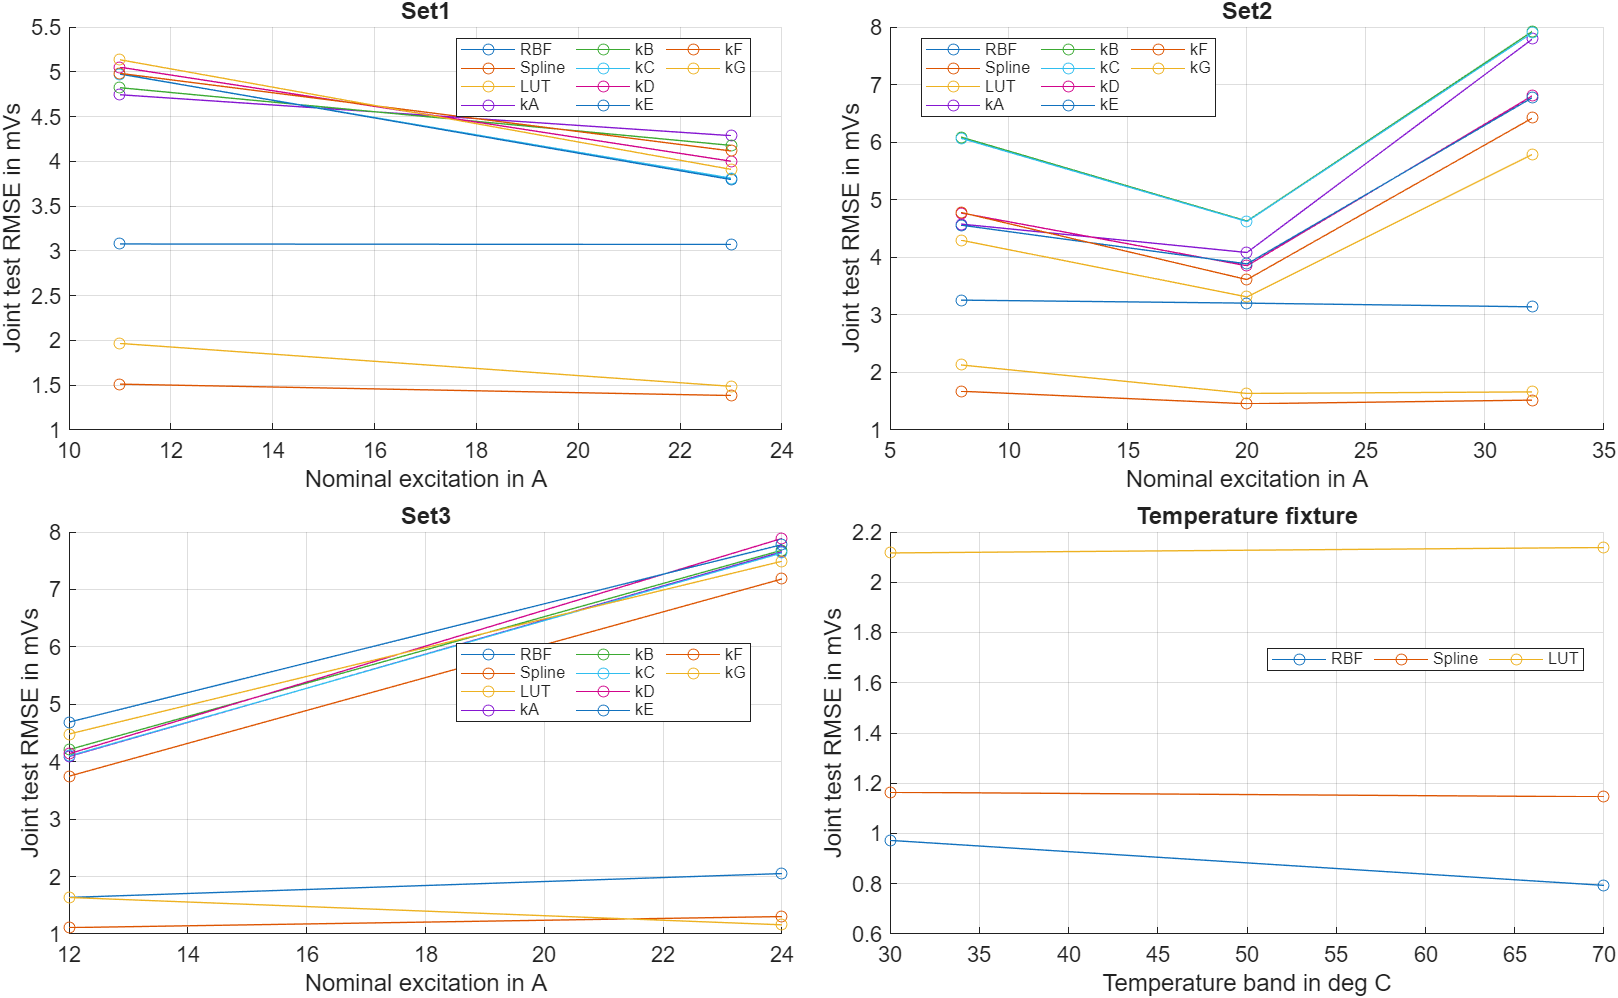
\includegraphics[width=\linewidth]{group_errors.png}
\caption{Joint test error by excitation group. Dataset 4 uses spatial holdout within both temperature bands; no independent temperature holdout is implied.}\end{figure}
\subsection{Reconstruction and representation difference}
The next table reports joint reconstruction error in mVs on common final-training points. It is a fit-to-available-data diagnostic, not independent prediction.
\begin{center}\ReconstructionTable\end{center}
The following are joint differences from the fresh full LUT in mVs, not errors against physical truth.
\begin{center}\DifferenceTable\end{center}
\begin{figure}[htbp]\centering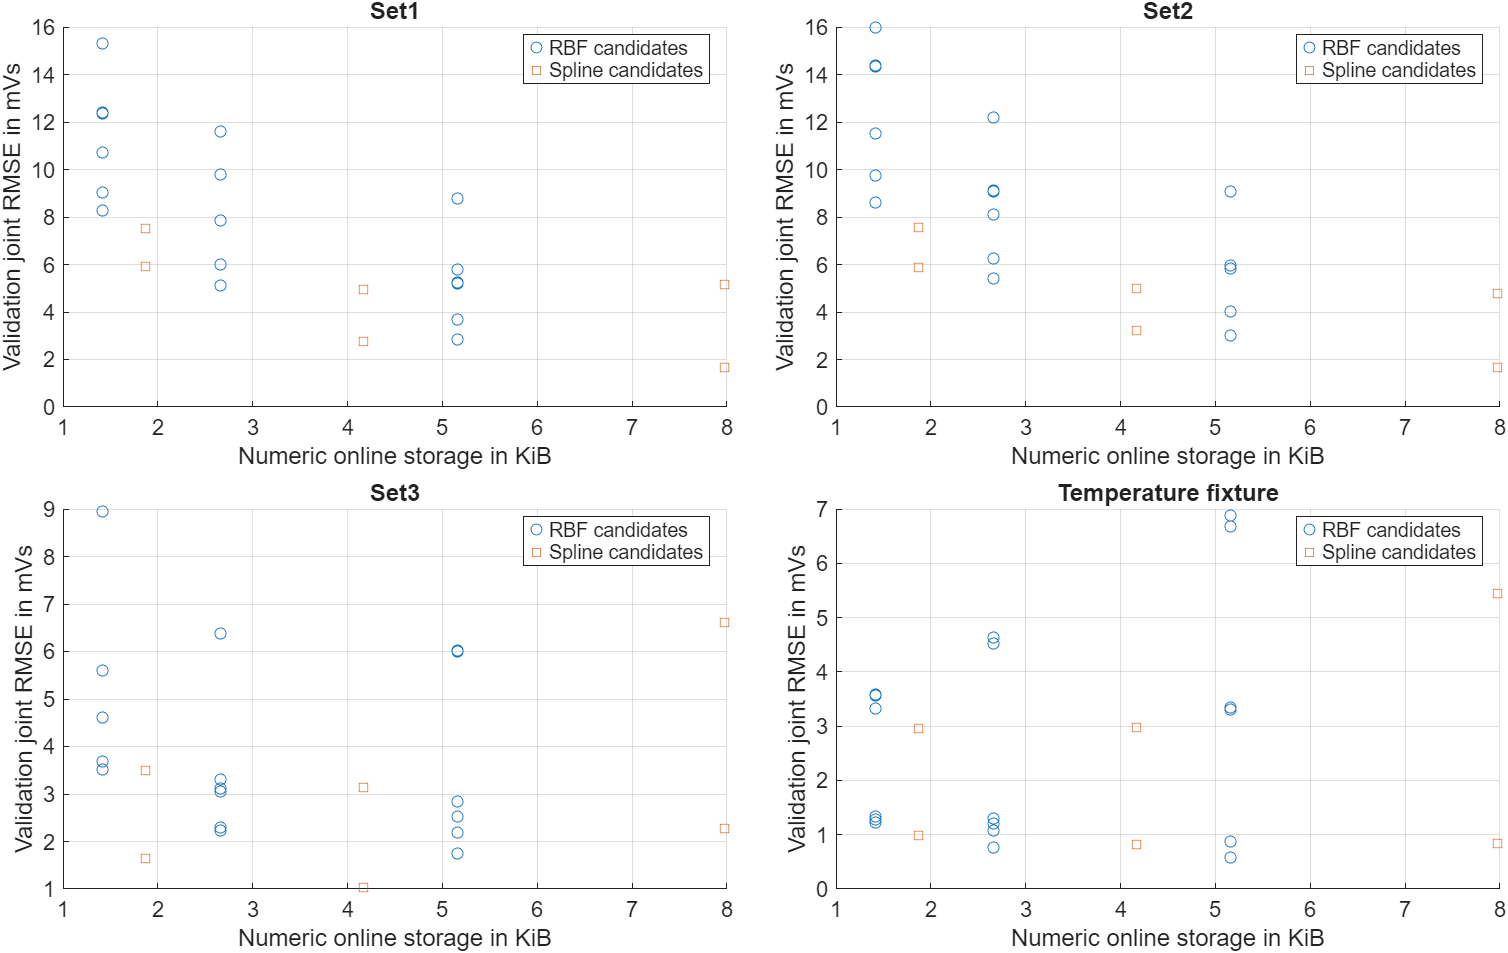
\includegraphics[width=\linewidth]{size_error.png}
\caption{Configured storage/validation-error comparison. Width and ridge choices produce multiple candidates at each size. Test errors do not determine selection.}\end{figure}
\begin{figure}[p]\centering
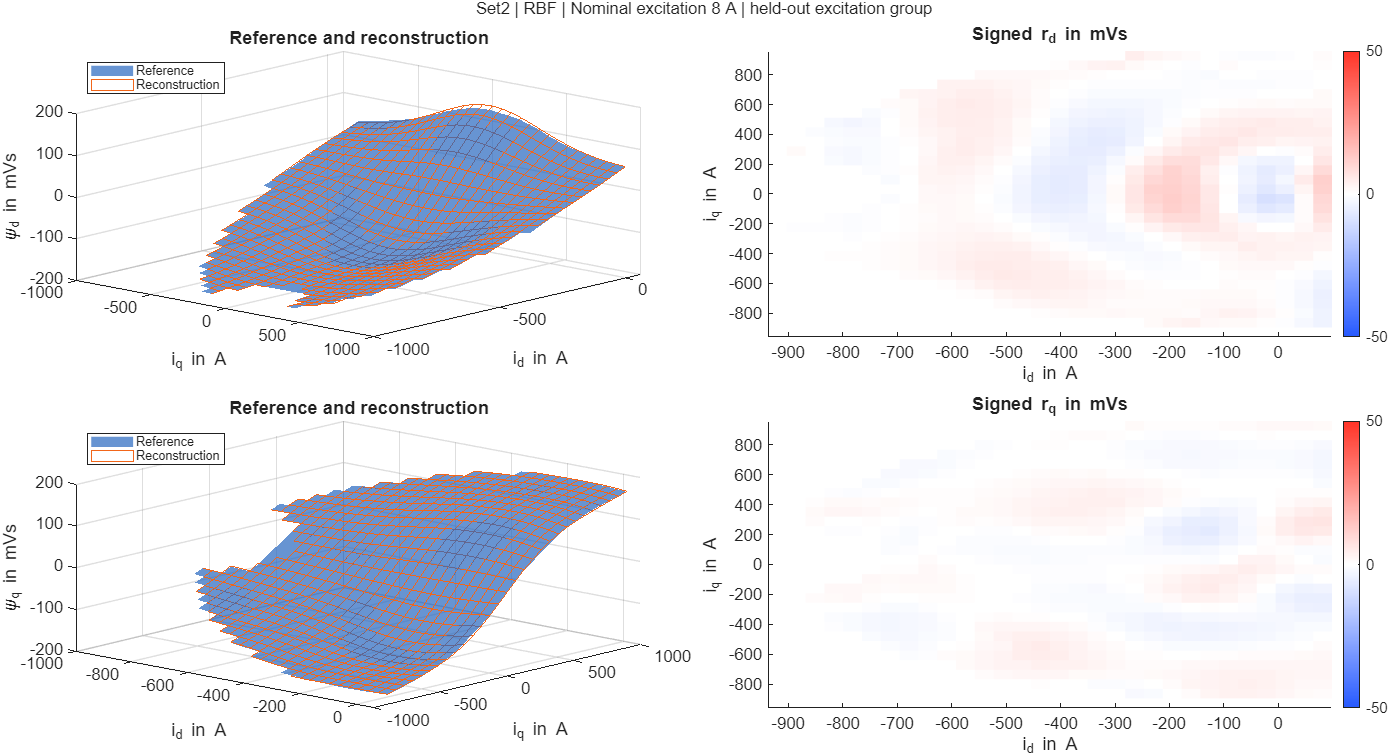
\includegraphics[width=\linewidth,height=.38\textheight,keepaspectratio]{example_rbf.png}
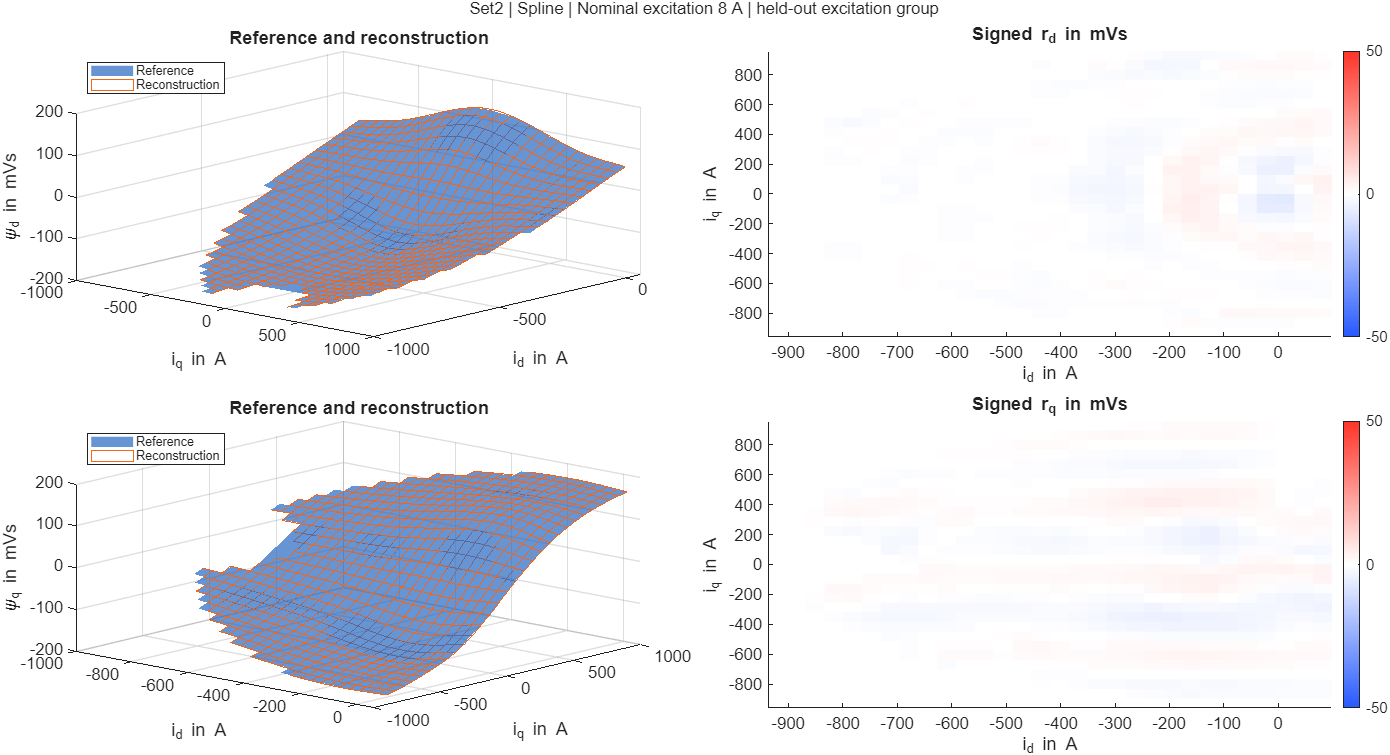
\includegraphics[width=\linewidth,height=.38\textheight,keepaspectratio]{example_spline.png}
\caption{Held-out Set 2 group: RBF above, spline below. References are blue, reconstructions orange. Signed errors retain physical d/q order; the d-flux 3D axes are exchanged for visibility. White regions lack common support. Display grids differ from numerical test points.}\end{figure}
\FloatBarrier
\subsection{Derivative disagreement}
RMS differences below are in mH relative to 80-neighbor training-derived slopes at identical test points. They are diagnostics, not independent inductance measurement errors.
{\small\DerivativeTable}
Dataset 4 current derivatives use mH; its temperature derivative differences use mVs/K in the CSV. A smooth fit and noisy local slopes may disagree without disproving the fit physically. Small flux errors alone do not establish derivative accuracy.

\subsection{Storage and PC cost}
Numeric storage counts mandatory double arrays: coefficients/nodes, centers/widths or knots, normalization, coordinate parameters and box bounds. Offline training indices, textual provenance, MATLAB overhead, work arrays and an additional geometric guard are excluded. Research structures include those offline items; their MATLAB byte counts are also exported.

Every timing uses two fluxes, six physical first derivatives and validity work at one scalar query. After scalar warm-up, seven batches each cycle through the same twelve supported queries ten times. The median is a per-call batch-average median; even the maximum batch average is not worst-case single-call latency.
{\small\CostTable}
These PC/MATLAB results compare supplied prototypes. Dispatch, sparse construction, exponentials, interval search, compilation and numeric precision can change target-hardware rankings.

\section{Controller, exact reuse and 20 kHz}
The inspected principal current-controller branch receives main d/q current requests, not measured current feedback. It evaluates a flux pair at main requests and another at the d request plus an additional d-current term, with q unchanged. Four d/q inductance outputs use that summed-current point. The local wrapper thus has three input quantities and eight outputs: two flux pairs and four inductances. Internal port names suggesting filtered measurements do not change the traced request signals.

The research package is one physical query with all three-input derivatives. The complete existing wrapper needs two operating-point evaluations and does not expose temperature/excitation as independent local inputs. Their complete replacement cost cannot be inferred by equating these packages. The requests are tapped at the current-controller inlet before the local additional d-current sum. Concrete paths and signal tags are in the technical note.

Exact reuse by a deterministic static evaluator requires an unchanged complete query tuple, parameter/model revision, interpretation mode and validity policy. Fluxes, derivatives and validity can then be reused together. LUTs can use the same mechanism. An unchanged torque request does not prove unchanged current requests, temperature, excitation or added-current terms. No controller trace was recorded to measure cache hit rate.

A tolerance rule for changed inputs is approximate. A local $J\Delta\bm x$ estimate alone does not establish a uniform error bound. No cache or tolerance rule is enabled in production.

At 20 kHz the entire task period is $50\,\mu$s, not the free evaluator budget. A hardware decision needs the actual hardware/compiler, complete task profile, required output package, numeric precision, domain-check cost, update-tick latency and interference allowance. Reuse can reduce average cost but cannot excuse an over-budget update tick.

\section{Recommendation and limitations}
Within the configured candidates and supported excitation tests, the cubic spline is the first candidate for a target-hardware prototype: it retains all three physical inputs with a small coefficient package and is competitive with the full LUT in measured-reference flux error. This is a candidate-selection recommendation, not universal spline superiority or validated application accuracy.

The Gaussian model remains an appropriate timing comparator. Its MATLAB evaluator directly shares exponential values between outputs and derivatives; the PC ranking need not survive a compiled local-spline implementation. The search is limited to deterministic centers, a common width and at most 128 centers. It does not exhaust the RBF design space.

The k representations impose a coordinate-reduction constraint that coefficient compression does not require. A different group split can change their ranking; results are recalculated here rather than transferred from another experiment. Differences from fresh or pre-existing LUTs are not causal error partitions.

No final controller-replacement decision is justified. Missing evidence includes application limits for flux and derivative errors, independent derivative/thermal validation, and target-hardware timing of the actual two-operating-point package with its guard and numeric precision. Temperature was not controlled in the current campaigns, and the secondary artifact cannot close that gap. The sampled sizes, one predetermined partition, restricted coverage and finite k-search budgets limit generalization. No production controller was changed.

\appendix
\section{Reproduction and companion material}
The execution note records file/function references, split rules, model packages and commands. MAT models save active inputs/units, fixed-condition descriptions, normalization, bounds, basis parameters, coefficients and training identities. Comparison scripts reload saved models without fitting coefficients. The starter rebuilds preparation, fits, comparisons and figures.

The atlas shows every group and applicable method. Axes/captions remain English, with quantities labelled in A and in mVs. Source triangles preserve gaps; the third measured input is interpolated with fluxes for display queries. Reconstruction/error maps use common support, while numerical metrics remain point-based. This intersection can mask otherwise finite coefficient predictions, including training boundary slices without complete LUT cells. No production controller or existing k-factor manuscript is changed.
\end{document}
